%!TEX root = ../main.tex
%%%%%%%%%%%%%%%%%%%%%%%%%%%%%%%%%%
% Links:
%
% Difficulty: Companies: 
%%%%%%%%%%%%%%%%%%%%%%%%%%%%%%%%%%

\chapter{Number of Dice Rolls With Target Sum}
\label{ch:dice_rolls}
\section*{Introduction}

Dices have been around for quite a long time: the oldest dice known  were discovered in Iran, as part of a staggering five-thousand-year-old
 Backgammon\footnote{One of the oldest board game. A two-players game where pieces are moved around between twenty-four triangles according to the roll of two 6 faced-dice. The goal of each player is to remove all of their 15 pieces before the other player} set.

If we think about what a die is, the first thing that comes to mind is the fair $6$ faced-die (see Figure \ref{fig:dice_rolls:6faces_dice}), but potentially any polyhedron can be a die: consider for instance a  $20$-faced icosahedron (see Figure
\ref{fig:dice_rolls:20faces_dice}), or a $12$-faced dodecahedron (see Figure
\ref{fig:dice_rolls:12faces_dice}).
In this chapter's problem, we will use up to $30$ dice at the same time,
each with up to $30$ faces, and we are going to calculate the number of ways we can obtain a certain
target value when we throw them all at the same time.


\section{Problem statement}
\begin{exercise}
You have $d$ dice, and each die has $f$ faces numbered $1, 2, \ldots..., f$.
Write a function that returns the number of possible ways to roll the dice
so the sum of the upper
faces equals a given target number $t$. Because this number can be very large, the answer
should be returned modulo $10^9 + 7$.
	

	\begin{example}
		\hfill \\
		Given $d=1$, $f=6$ and $t=6$ the function should return $1$. Clearly, there is only one way to obtain $6$ when rolling a common $6$-face cubic die.
	\end{example}

	\begin{example}
		\label{ex:dice_rolls:example2}
		\hfill \\
		Given $d=2$, $f=6$ and $t=7$ the function should return $6$. Table \ref{tab:dice_rolls:arrangements_example2} lists all the possible ways of obtaining $7$ from two common $6$-face dice.
	\end{example}

	\begin{example}
		\hfill \\
		Given $d=2$, $f=3$ and $t=7$ the function should return $0$ because the highest number	obtainable by rolling two dices with three faces is $6$.
	\end{example}
\end{exercise}

\begin{table}
	\centering
	\begin{tabular}{|c|c|} 
	\hline
	\textbf{First die} & \textbf{Second die}  \\ 
	\hline
	1                  & 6                    \\
	2                  & 5                    \\
	3                  & 4                    \\
	4                  & 3                    \\
	5                  & 2                    \\
	6                  & 1                    \\
	\hline
	\end{tabular}
	\caption{Possible valide arrangements of two dice for the Example \ref{ex:dice_rolls:example2}}
	\label{tab:dice_rolls:arrangements_example2}
\end{table}


\section{Clarification Questions}

\begin{QandA}
	\item What is the maximum number of dices, faces, and the highest target value possible?
	\begin{answered}
		$30$,$30$ and $1000$, respectively.
	\end{answered}
	
\end{QandA}

\begin{figure}
	\centering
	\begin{subfigure}[t]{0.25\textwidth}
		\includegraphics[width=1\linewidth]{/home/dspataro/git/algorithm_articles/sources/dice_rolls/images/3d_dices}
		\caption{Example of dice with $12$ faces.}
		\label{fig:dice_rolls:12faces_dice}
	 \end{subfigure}
	\hfill
	\begin{subfigure}[t]{0.25\textwidth}
		\includegraphics[width=1\linewidth]{/home/dspataro/git/algorithm_articles/sources/dice_rolls/images/cubic_dice}
		\caption{Example of common $6$ faces dice.}
		\label{fig:dice_rolls:6faces_dice}
	 \end{subfigure}
	 \hfill
	 \begin{subfigure}[t]{0.25\textwidth}
		 \includegraphics[width=1\linewidth]{/home/dspataro/git/algorithm_articles/sources/dice_rolls/images/icosahedron_dice}
		 \caption{Example of dice with $20$ faces.}
		 \label{fig:dice_rolls:20faces_dice}
	  \end{subfigure}
\end{figure}

\section{Discussion}
\label{dice_rolls:sec:discussion}

Let's start by noticing that the answer can be astronomically high, but more importantly, the number of possible value combinations resulting from rolling $d$ dices is even larger: if each die has
$f$ faces, then we are looking at $f^d$ possible distinct roll outcomes! 
During an interview, a brute-force approach, where we go over each and every possible roll outcome of the $d$ dice, is completely out of question  (considering the constraints on the maximum number of dices and faces we might get for input) unless we are willing to wait around  $6 \times 10^{18}$ years. Even if we implement this algorithm so that it can run on the fastest supercomputer available today (which is capable of a staggering $\approx450$ \footnote{\textbf{petaflop}: A petaflop is a measure of a computer's processing speed and can be expressed as: A quadrillion (thousand trillion) floating-point operations per second (FLOPS). A thousand teraflops. 10 to the 15th power FLOPS. 2 to the 50th power FLOPS. A huge number of operations per second.} operations per second), it would still require $\frac{30^{30}}{10e15}$s to run to completion. By that time, humanity will be long gone, the universe will be a dark and cold place, but most importantly, the position you are dreaming about will have gone to somebody else.

This type of \textit{"counting"} questions is usually (and crucially more efficiently) solved by using a dynamic programming
approach. In fact, this question shares a lot of similarities with the classical dynamic programming
\textit{Coin change} problem, to the point that we
could solve this one using the solution to the other. In fact we can stretch this reasoning so to consider the topic treated in this chapter to be a proper specialization of the *Coin
change* problem, where the number of available coins is equal to $d$
and the denomination of the coins are $1,2,\ldots,f$: we have coins of the same denomination as the
dice faces.




\subsection{Brute-force}
\label{dice_rolls:sec:bruteforce}


For science's sake, let's see how a brute-force approach would apply here. As we all know, a brute-force approach evaluates all possible outcomes of rolling $d$ dice and keeps
track of how many yield a total sum of $t$. When dealing with this kind of task, where you have to
enumerate/generate the elements of a given set, recursion is usually the way to go, especially if the elements (in this case a combination of face values) have a recursive definition.
In this specific case, we can generate all possible combinations of $d$ faces we can obtain from rolling $d$ dices by:

\begin{itemize}
	\item generate the combinations from rolling $d-1$ dice;
	\item create $f$ copies of them;
	\item prepend $1$ to the items of the first copy;
	\item prepend $2$ to the items of the second copy;
	\item $\ldots$  
	\item prepend $f$ to the items of the last copy.
\end{itemize}


For instance, we can generate all rolls outcome $3$ six-faced dice by:

\begin{enumerate}
	\item Generate all the outcomes for only $2$ of them $C_2$:\\
	$
	\!
	\begin{aligned}[t]
		C_2 =  \{
			& (1,1),(1,2),(1,3),	(1,4),	(2,1),	(2,2),	(2,3),	(2,4),\\
			&(3,1),	(3,2),	(3,3),	(3,4),	(4,1),	(4,2),	(4,3),	(4,4)\}
	\end{aligned}
	$ 
	

	\item Append $1$ to each of the elements of $C_2$:\\
	$
	\!
	\begin{aligned}[t]
		C_3^1 =  \{
			&(1,1,1),(1,1,2),(1,1,3),(1,1,4),(1,2,1),(1,2,2),(1,2,3),(1,2,4),\\
			&(1,3,1),(1,3,2),(1,3,3),(1,3,4),(1,4,1),(1,4,2),(1,4,3),(1,4,4)\}
	\end{aligned}
	$ 


	\item  Append $2$ to each of the elements of $C_2$: \\
	$
	\!
	\begin{aligned}[t]
		C_3^2 =  \{
			&(2,1,1),(2,1,2),(2,1,3),(2,1,4),(2,2,1),(2,2,2),(2,2,3),(2,2,4),\\
			&(2,3,1),(2,3,2),(2,3,3),(2,3,4),(2,4,1),(2,4,2),(2,4,3),(2,4,4)\}
	\end{aligned}
	$ 



	\item  Append $3$ to each of the elements of $C_2$:\\
	$
	\!
	\begin{aligned}[t]
		C_3^3 =  \{
			&(3,1,1),(3,1,2),(3,1,3),(3,1,4),(3,2,1),(3,2,2),(3,2,3),(3,2,4),\\
			&(3,3,1),(3,3,2),(3,3,3),(3,3,4),(3,4,1),(3,4,2),(3,4,3),(3,4,4)\}
	\end{aligned}
	$ 
	\item Prepend $4$ to each of the elements of $C_2$:\\
	$
	\!
	\begin{aligned}[t]
		C_3^4 =  \{
			& (4,1,1),(4,1,2),(4,1,3),(4,1,4),(4,2,1),(4,2,2),(4,2,3),(4,2,4),\\
			&(4,3,1),(4,3,2),(4,3,3),(4,3,4),(4,4,1),(4,4,2),(4,4,3),(4,4,4)\}
	\end{aligned}
	$ 

	\item  Finally, return $C_3 = \{C_2^1 \cup  C_2^2 \cup C_2^3 \cup C_2^4\}$
	
\end{enumerate}


The definition above is correct, but not very useful in practice: it requires making many copies
of a potentially very large (indeed exponential) set of items. We will therefore use a different approach that will still run in exponential time (this section is named brute-force after all), but it can be used as a basis for developing a more efficient DP solution.

We start by rolling the first die; clearly, we have $f$ possible values we can get, but
once the value for this specific die is set, say we got the value $x$, we are left with $d-1$ dices
to roll and we still have to make up for $t-x$ with the remaining $d-1$ dice in order to reach our target value
$t$. 
Once a die is rolled, we are left with exactly the original problem on a smaller number of dice
and target value. 
This is why recursion is handy as we can describe the solution to the entire problem in terms of solutions to
sub-problems.
We can continue this recursive process, rolling one die at a time, until we reach one of the following cases:
\begin{enumerate}
	\item $d<0$ or $t<0$ the answer is $0$. There is no solution to the problem when the number of
		dice to use is negative or the target number is negative.
	\item $t=0$. We have reached the target value $t$. If we have used \textbf{all} dice then we
		have a solution, otherwise we do not. In other words:
	\begin{itemize}
		\item  if $d=0$, we have used all $d$ dice and the sum is exactly equal to $t$. This is a
		valid combination. We have rolled $d$ dice and the sum of their faces is exactly equal to
		$t$.
		\item if $d>0$, we have not rolled all the dice, yet we have already reached our target
		value. If we continue to roll, we will generate a combination with a total sum higher than
		$t$. This is not a good combination.
	\end{itemize}
\end{enumerate}

The idea above can be better expressed using the recurrence relation shown in Equation
\ref{eq:dice_rolls:dpformula} where $S(d,t,f)$ is the number of ways one can obtain a target value
$t$ by throwing $d$ dice. Notice that the third parameter never changes, and thus it does not play a
dynamic role in the recurrence. 

\begin{equation}
	S(d,t,f)=\begin{cases}
		 1 \: \: \text{ if } \: d=t=0 \\
		 0 \: \: \text{ if } \: d=0, \: t>0 \\ \\
		\sum_{1}^{\min(f,t)} S(d-1,t-j,f)  \:\: \text{ otherwise}
	 \end{cases}
	\label{eq:dice_rolls:dpformula}
\end{equation}

Listing \ref{list:dice_rolls:bruteforce} shows a possible implementation of such idea. Please note
that this code is remarkably similar to the brute-force solution for the Coin Change problem in
Chapter \ref{ch:coin_change}. Section
\ref{sec:min_difficulty_job_scheduler:generate_all_combination} also discuss the problem of
generating combinations, and the material discussed there can be adapted and applied here.

\lstinputlisting[language=c++, caption={Brute-force (enumerating all possible combinations) solution for the problem of counting the number of dice rolls summing up to a target number $t$.},label=list:dice_rolls:bruteforce]{/home/dspataro/git/algorithm_articles/sources/dice_rolls/dice_rolls_solution1.cpp}


The time and space complexity of this approach are exponential and constant, respectively.
 
The proof of this  can be derived from the solution of the recurrence relation shown in Equation \ref{eq:dice_rolls:dpformula_complexity}:
\begin{equation}
	S(d,t) = S(d-1,t-1) + S(d-1,t-2)
\label{eq:dice_rolls:dpformula_complexity}
\end{equation}

where $S(d,t)$expresses the number of invocations of the function 
\inline{num_rolls_to_target_bruteforce}
for a given number of dice $d$ and target value $t$ when $f=2$. 
The resulting invocation tree is
complete and has height $h=t$ (assuming $d \leq t$, but the same reasoning can be applied in the
other cases). 
The cost of each node of the tree is $O(1)$. The number of nodes in such a tree is
exponentially proportional to its height. 



\subsection{Dynamic Programming - Recursive top-down}
\label{dice_rolls:sec:DP}
The brute-force solution we laid down in Section \ref{dice_rolls:sec:bruteforce} can  be turned into a nice and
efficient one with the help of DP, and in particular of memoization. As per many other problems
solvable with DP out there, the brute-force solution above can be turned into a much more
efficient one by simply realizing that the same sub-problems are solved over and over again.
For istance, imagine the case where $f=5$. We might end up solving the sub-problem where $d=1$ and
$t=3$  from the sub-problem where $d=2$, $t=4$ (by rolling the face with $1$), or from the
sub-problem $d=2$, $t=5$ (by rolling the face with $2$).

However, the maximum number of \textit{distinct} invocations for the function
\inline{num_rolls_to_target_bruteforce} is not larger than $30\times 1000 = 30000$: the maximum number of dice multiplied by the largest target value as these are the only function parameters varying during the execution. If we can somehow guarantee that no
duplicate work is done for a given $d$ and $t$, then we can get away with only $O(d\times t)$
function calls. 

Consider, for instance, what happens during the execution of the code
in Listing \ref{list:dice_rolls:bruteforce} for the following input:
\begin{itemize}
	\item $d = 3$
	\item $f = 6$
	\item $t = 12$
\end{itemize}


The function \inline{num_rolls_to_target_bruteforce(1,5,6)} is called  $6$ times and the
sub-problem \inline{num_rolls_to_target_bruteforce(1,4,6)} is solved $5$ times.
You can verify this yourself if you draw the recursion tree for \inline{num_rolls_to_target_bruteforce(3,6,12)}, or simply add a print statement at the beginning of the function.
All these duplicate calls are superfluous and they represent work that can be saved if the result of each sub-problem is stored into a
cache as shown in the following Listing.


The function subproblem \inline{num_rolls_to_target_bruteforce(1,5,6)} solved $6$ times and the
subproblem \inline{num_rolls_to_target_bruteforce(1,4,6)} is solved $5$ times. If you are not
convinced draw the recursion tree, or add a print statement at the beginning of the function. All
these superfluous execution can be avoided if the result of each of the subproblem is stored into a cache as shown in Listing \ref{list:dice_rolls:dp}. 

\lstinputlisting[language=c++, caption={Dynamic programming with memoization top-down recursive  solution for the problem of counting the number of dice rolls summing up to a target number $t$.},label=list:dice_rolls:dp]{/home/dspataro/git/algorithm_articles/sources/dice_rolls/dice_rolls_solution2.cpp}


This implementation is an almost identical copy
of the brute-force solution, except for the addition of a cache. Note how \textbf{before} actually trying
to compute the answer, we first look into the cache (see highlighted lines) to see if it is already present in the cache. If not, we solve the
problem and before returning the answer we \textbf{save} the result into the cache.

\section{Dynamic programming - Iterative bottom-up}
\label{dice_rolls:sec:bottom}

Turning the top-down-up solution shown in Section \ref{dice_rolls:sec:DP} into a bottom-up one is relatively easy: the recursive
definition of the solution (see Equation \ref{eq:dice_rolls:dpformula})   clearly shows that we can
calculate the answer for a given number of dice $d$ and a target value $t$ if we have already
calculated the values for targets $t-1, t-2, \ldots, t-f$ and $d-1$. We also know how to easily
calculate the answer for all possible target values when $d=0$ and $d=1$ and from there we can apply
the reasoning above. 
This is exactly the strategy that Listing \ref{list:dice_rolls:dpbottomup} implements.

\lstinputlisting[language=c++, caption={Dynamic programming bottom-up solution for the problem of counting the number of dice rolls summing up to a target number $t$.},label=list:dice_rolls:dpbottomup]{/home/dspataro/git/algorithm_articles/sources/dice_rolls/dice_rolls_solution3.cpp}

We use a 2D
table \inline{DP} (initialized with zeros) with $d+1$ rows and $t+1$ columns where each cell \inline{DP[i][j]}
corresponds to the solution of a sub-problem where $d=i$ and $t=j$. The first loop takes care of
filling the table with \textit{"known" values} for all sub-problems where $d=1$. If we only have a die with
$f$ faces, there is only one way we can achieve the target values $1,2,\ldots, f$ and no way to
obtain any higher values. The rest of the code fills the table one row at a time (one dice at a
time) by using the values of the previous row. 

The time and space complexity of this algorithm are $\Theta(dtf)$ and $\Theta(dt)$, respectively. 
However, the space complexity can be lowered easily
down  to $\Theta(t)$ because, as already mentioned, we only need space for two rows of the DP table:
one for the values of the current $d$ and one for the values at $d-1$.
